\subsection{Keypoint-Based Visual SLAM}
\label{sec:kv_slam_background}

SLAM is the joint problem of simultaneously generating a map of an environment and estimating the position of an observer within that map based on sensor observations. First explored in the 1980s \cite{smithEstimatingUncertainSpatial1988}, SLAM has become a de facto standard in robotics for tasks which require operations within unfamiliar environments. A wide variety of sensors can be utilized by SLAM, the most common being LiDAR, cameras, and RGBD sensors. The high level relationships between these sensor modalities are shown in Figure \ref{fig:slam_family_tree}. Keypoint-Based Visual SLAM (KV-SLAM) refers to a subset of the wider SLAM ecosystem characterized by the use of cameras as the primary sensor, and image features extracted from images as the primary data for tracking and mapping.

\begin{figure}[!ht]
    \centering
    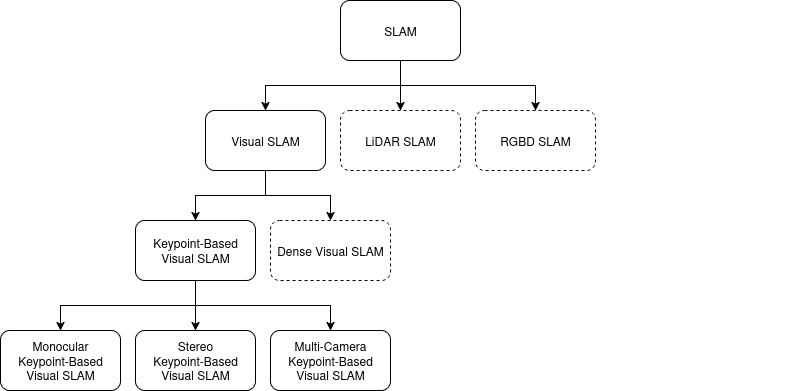
\includegraphics[width=0.9\textwidth]{resources/slam_family_tree.png}
    \caption[SLAM Family Tree]{Overview of the relationships between popular SLAM modalities.}
    \label{fig:slam_family_tree}
\end{figure}

The first implementations of KV-SLAM came in the early 2000s \cite{seMobileRobotLocalization2002}\cite{davisonRealtimeSimultaneousLocalisation2003}, making the field relatively young. This can be attributed to the difficulty in estimating 3D geometries from 2D images, unlike LiDAR and RGBD which are capable of direct 3D environmental measurements. However, due to the extremely low cost and wide availability of camera sensors, KV-SLAM is a popular modality for robotics, AR/VR, and autonomous driving applications. This research ties into to the structures and inner workings of KV-SLAM systems, so an overview of the concepts and techniques used in KV-SLAM is provided below.

\subsubsection{Image Features}

An image feature is the combination of a keypoint and a feature descriptor \cite{loweObjectRecognitionLocal1999}. Keypoints are locations in an image which are designed to be invariant to lighting, scale, translation, and rotation, while descriptors are a data vector that acts as a unique fingerprint for a feature. Keypoints are located, and their descriptors generated in a process called feature extraction.

Image features can be matched between frames using their descriptors. For many features such as SIFT \cite{loweObjectRecognitionLocal1999}, SURF \cite{baySURFSpeededRobust2006}, and ORB \cite{rubleeORBEfficientAlternative2011}, the descriptor is a vector of floating point values, calculated from pixel values surrounding the keypoint, which can be compared using a distance metric such as Euclidean distance or Hamming distance.

The purpose of feature extraction is to reduce the large input image data to a small set of easily detectable and trackable features, allowing the huge majority of the image data to be discarded. Figure \ref{fig:feature_extraction_and_matching} shows the output of the ORB feature extractor on two input images, and the matching features between the two images. The capability to match the same set of points across multiple viewpoints is core to how 3D map points are estimated from multiple 2D images.

\begin{figure}[!ht]
    \centering
    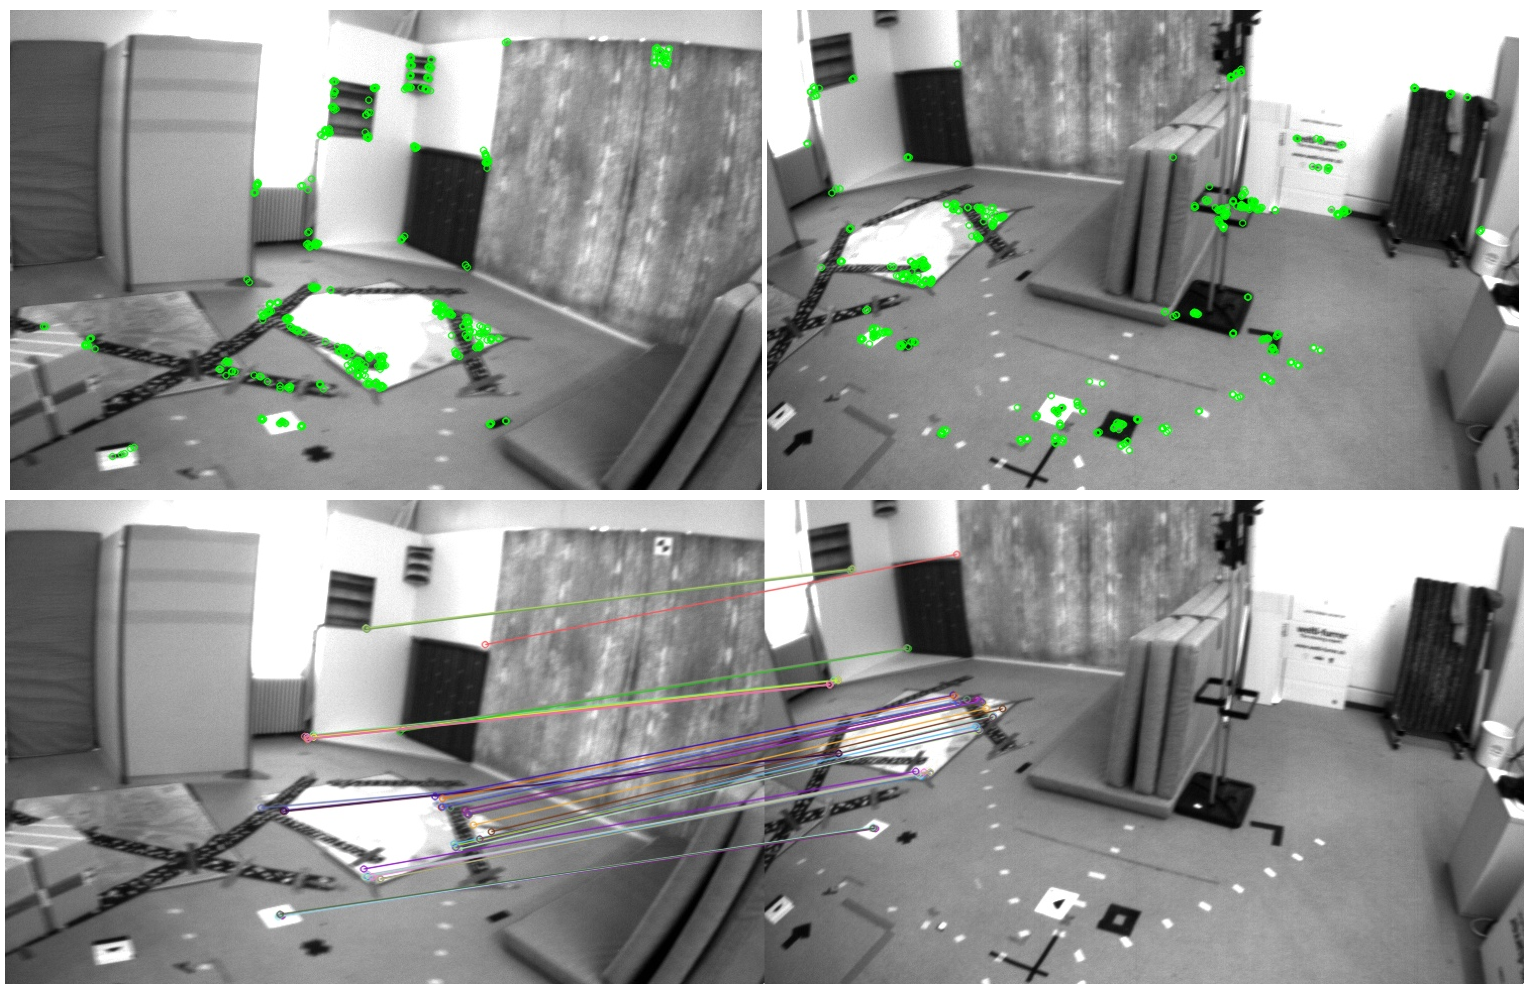
\includegraphics[width=0.9\textwidth]{resources/feature_extraction_and_matching.png}
    \caption[Image Feature Extraction and Matching]{(Top) ORB features extracted from two frames of the EuRoC MAV V1\_03 dataset \cite{burriEuRoCMicroAerial2016}. (Bottom) Corresponding ORB feature matches between the two frames.}
    \label{fig:feature_extraction_and_matching}
\end{figure}

\subsubsection{Robust Estimation and RANSAC}

Image feature matching is a noisy process, meaning the correspondences between features in different images will not always be correct. This is especially true when the environment contains repetitive patterns. To address this, robust estimation techniques are used to filter outliers from the data. In the context of KV-SLAM, the most common robust estimation technique is called Random Sample Consensus (RANSAC) \cite{fischlerRandomSampleConsensus1981}.

RANSAC is an iterative algorithm that estimates model parameters from a dataset containing outliers. It works by randomly selecting a subset of the data, fitting the model to this subset, and then counting the number of inliers that fit the model within a certain threshold. The process is repeated until a model is found that matches a sufficient number of inliers, or a maximum number of iterations is reached.

Figure \ref{fig:ransac} provides a visual representation of the process RANSAC takes to fit data with outliers. If one were to sample linear data with a noisy sensor that sometimes produces outliers, the output may look like the left most plot of the figure. As can be seen, the best fit line is severely skewed by the outliers. By iteratively selecting a random sample of the input data, fitting the model to this sample, and counting the number of inliers, RANSAC can find a solution which explains a high proportion of the observations.

\begin{figure}[!ht]
    \centering
    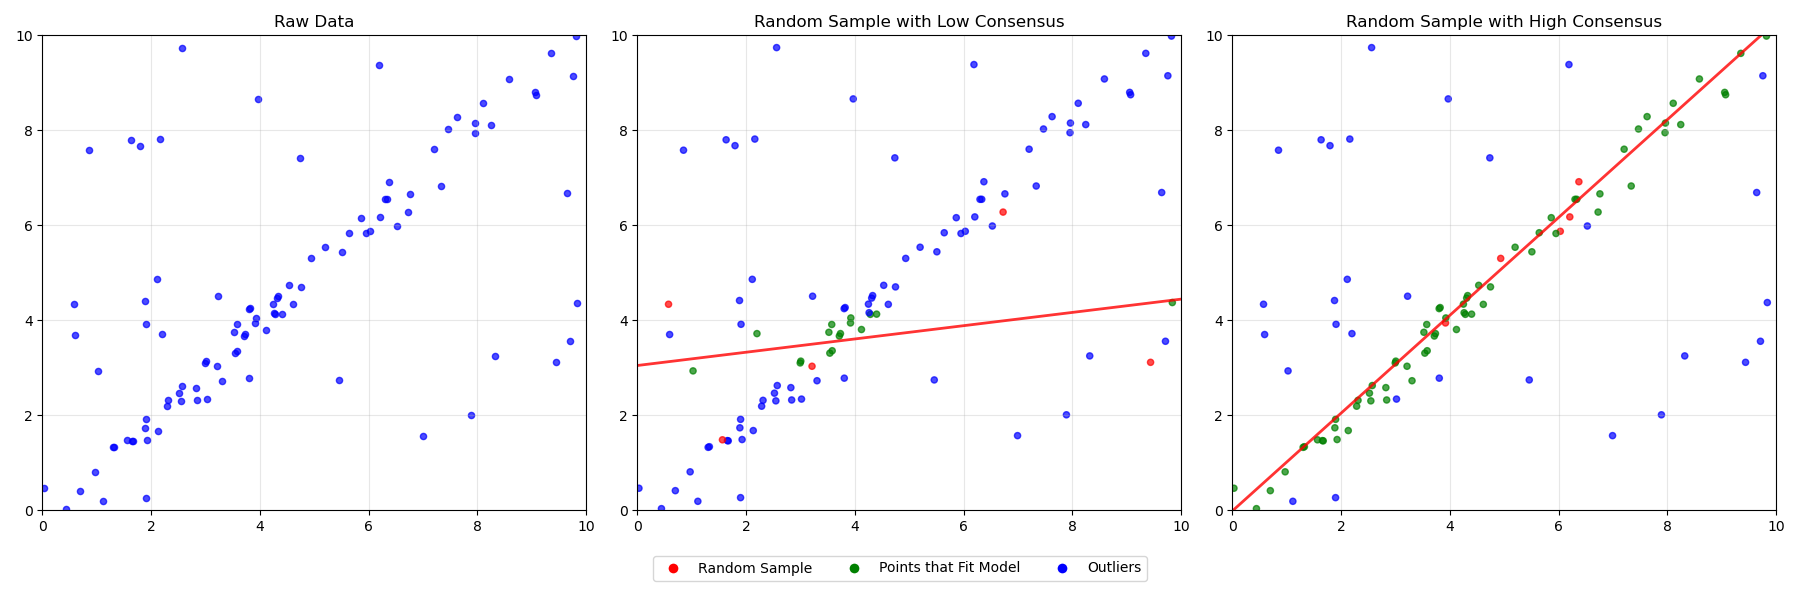
\includegraphics[width=0.9\textwidth]{resources/ransac.png}
    \caption[2D RANSAC Example]{A demonstration of how RANSAC determines model parameters through iterative random sampling and model application.}
    \label{fig:ransac}
\end{figure}

It should be noted that RANSAC requires a low proportion of outliers in the data to be effective, as it relies on randomly selecting a set of inliers for model fitting. For that reason, preprocessing steps which reduce the number of potential outliers in sample data are useful for improving the speed and effectiveness of RANSAC.

\subsubsection{Tracking and Mapping}

In the context of KV-SLAM, tracking refers to the process of estimating the real-time position and orientation of the camera, while mapping refers to the process of generating a 3D map of the environment. Methods like the eight-point algorithm can be used to simultaneously calculate the transformation and depths between two images taken from different viewpoints using their 2D-2D feature correspondences \cite{longuet-higginsComputerAlgorithmReconstructing1981}\cite{hartleyDefenseEightpointAlgorithm1997}. This is primarily used for map initialization, before any 3D map points have been established. Once a set of 3D map points have been established, tracking can be achieved using the Perspective-n-Point (PnP) algorithm \cite{fischlerRandomSampleConsensus1981}, with mapping utilizing triangulation to generate new map points \cite{davisonRealtimeSimultaneousLocalisation2003}.

Incorrect 2D-2D and 2D-3D correspondences degrade the performance of the tracking and mapping processes. To account for outliers in the correspondences, RANSAC is used to estimate the transformations and 3D depths on a subset of the matches with the goal of finding a transformation which maximizes the number of correspondence inliers.

In the context of this research, the 2D-3D correspondences between an image and the map may contain more outliers when the map contains a significant number of outdated map points. If this conjecture is true, an improvement in the speed and robustness of the RANSAC process should be seen after the implementation of the proposed VD-MPR method.

\subsubsection{Loop Closure and Relocalization}

Loop closure is a technique used to correct drift during large scale KV-SLAM operations \cite{cumminsProbabilisticAppearanceBased2007}. The process works by recognizing when the system has entered a previously visited place, usually by detecting visual similarity between this place and the current image. Due to noise inherent to the system, the current position estimate may not match the position estimate from the previous visitation. The drift error is simply the difference between the previous and current position estimates, and can be propagated through the historical trajectory estimations, re-aligning the two positions. Figure \ref{fig:loop_closure} shows how loop closure identifies a previously visited place, and corrects the trajectory to remove accumulated drift.

\begin{figure}[!ht]
    \centering
    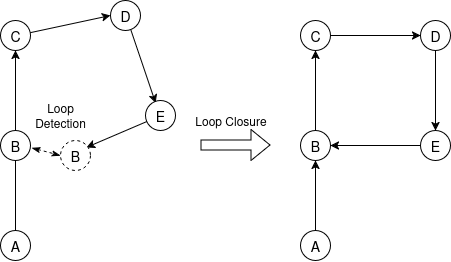
\includegraphics[width=0.9\textwidth]{resources/loop_closure.png}
    \caption[Loop Closure Example]{An example of how loop closure can correct drift by constraining the trajectory based on detected loops.}
    \label{fig:loop_closure}
\end{figure}

Relocalization is used when the SLAM system is "lost", meaning a map of the environment exists, but the location of the camera within this map is unknown. This can happen for many reasons such as going through an area with low visual texture, dim lighting, or temporary obstruction of the camera by a moving object. To recover, the SLAM system looks for positions within the map which are visually similar to the current image. If a strong candidate position is found, the system attempts to find a valid pose for the image in the map using PnP and RANSAC.

Both of these operations rely on the ability to recognize visual similarity between the current image and the map. But as stated previous, the image data is discarded, meaning visual similarity must be recognized another way. In KV-SLAM systems, this is commonly accomplished using a Bag-of-Words model, which represents the map's feature descriptors as a collection of visual words, allowing the system to recognize previously visited places based on the presence of these words in the current image's feature descriptors \cite{galvez-lopezBagsBinaryWords2012a}.

For this research, the existence of outdated map points in the map may cause the Bag-of-Words model to produce false positives or negatives, leading to incorrect relocalization or loop closure detections. Removing these outdated features from the map and from the Bag-of-Words model should improve the performance of these operations, as the system will no longer be attempting to match against outdated features.

\subsubsection{Map Reuse}

Map reuse is core to this research, as it is what allows SLAM to operate in the episodic operating model. By loading a previously generated map into the SLAM system, we allow the system to operate in a known coordinate frame, and to maintain a consistent map of the environment. In the episodic operating model, the system is expected to operate in the same environment over long periods of time. By reusing maps, 